\documentclass[sigconf, screen, review, balance=false]{acmart}
% Target: WWW 2027 Demo Track; four pages including references, non-anonymous.
% Submission requirements: https://www2027.thewebconf.org/demos/
\acmConference[WWW '27]{The ACM Web Conference 2027}{May 10--14, 2027}{Dublin, Ireland}
\acmBooktitle{Companion Proceedings of the ACM Web Conference 2027 (WWW '27)}
\acmYear{2027}
\setcopyright{none}
\acmDOI{}
\acmISBN{}
\usepackage{graphicx} % Required for inserting images
\usepackage{xurl}
\usepackage{colortbl}
\usepackage{hyperref}
\usepackage{needspace}
\newcommand{\BenchmarkQueryCount}{10000}
\newcommand{\BenchmarkCentroidSamples}{1000}

\graphicspath{{results/}{figures/}}

\title[Client-Side ANN on the Web]{Client-Side ANN on the Web: A Wikipedia Search Demonstration}
\author{David Denisov}
\affiliation{%
  \institution{University of Haifa}
  \city{Haifa}
  \country{Israel}
}

\begin{document}

\begin{abstract}
We demonstrate browser-based semantic search over $35.2$ million English Wikipedia passages served as static Web files. The browser embeds questions locally, uses inverted file (IVF) routing to select vector clusters for parallel download, ranks their vectors, and fetches text for the top results. This avoids a full index download or an application search server. Visitors can submit questions and inspect passages, timings, and download costs; a companion lab exposes the recovery--bandwidth trade-off. At 32k clusters, SQ6 centroids, and four probes, a fixed question returning ten passages averages $130.3$~ms, including embedding and text loading, with $3.25$~MB of compressed payload. Worker startup averages $2.46$~s. Controlled synthetic embedding perturbations yield $98.1\%$ source recovery. Queries and embeddings stay local, while file requests can reveal access patterns.
\end{abstract}

\ccsdesc[500]{Information systems~Similarity search}
\keywords{approximate nearest neighbors, semantic search, client-side retrieval}

\begin{teaserfigure}
\begin{minipage}{\textwidth}
\centering\small
\textbf{Live search demo:} \url{https://wiki-ann-demo-20261022.pages.dev/client_wiki/}\\
\textbf{Clustering lab:} \url{https://wiki-ann-demo-20261022.pages.dev/client_wiki/benchmark.html}\\
\textbf{Code and benchmarks:} see the accompanying repository.
\end{minipage}
\Description{Links to the live Wikipedia search demonstration and interactive clustering lab, with a reference to the accompanying source code and benchmark repository.}
\end{teaserfigure}

\maketitle


\section{Introduction}
Publishers can serve large document collections as static files, yet adding semantic search can require a search service or a large index download. Operating a search service adds deployment work; downloading the full index shifts transfer and storage costs to each visitor. We demonstrate approximate nearest neighbour (ANN) search over $35.2$ million Wikipedia passages using static Web hosting. Inverted file (IVF) routing selects clusters locally from downloaded centroids; the probe count determines how many clusters are fetched and searched.

At about $27$~GB of vectors, distributing our full index would impose a substantial initial download. Our contribution is the static-file deployment design: local IVF routing identifies candidate cluster files up front for independent parallel downloads while the full index stays remote. The search page and lab expose the costs of applying established ANN techniques at this scale. Cloudflare Pages hosts the client and sharded index.

\subsection{Related work}
Graph search, as in DiskANN~\cite{DiskANN}, discovers reads as traversal progresses. If graph data are served remotely, these dependencies can become successive network round trips. Browser-local \mbox{MeMemo}~\cite{MeMemo} and \mbox{WebANNS}~\cite{WebANNS} use HNSW with RAM and IndexedDB: an index is built or imported locally before queries, and graph traversal reads local storage. WebANNS evaluates up to $480{,}000$ passages ($7.5$~GB).

Our index stays remote. Startup downloads the model, runtime, and centroids (about $47$~MB); each query fetches selected vector files and result-text batches. IVF, implemented in Faiss~\cite{Faiss}, identifies all required cluster files locally, allowing parallel requests without waiting for remote graph expansion.

\section{Demonstration scenario}
\label{sec:demo}
The two public pages use the same Wikipedia passage collection.

\paragraph{Wikipedia search.}
Visitors enter a question or other text and receive ranked passages with links to Wikipedia articles. Defaults are 32k clusters, SQ6 centroids, four probes, and ten results. Controls offer three cluster counts, six centroid formats, and $1$--$100$ probes. The page reports embedding, centroid loading, retrieval, and text-loading times alongside vector downloads. Repeating a question with one and four probes reveals changes in results and download cost (Figure~\ref{fig:search-demo}).

\paragraph{Clustering lab.}
Visitors vary clustering, probes, centroid format, and query noise to compare recovery, downloads, and speed. The walkthrough uses 16k clusters, ten queries, one top match, and one versus four probes (Figure~\ref{fig:lab-demo}). Increasing probes exposes the recovery--bandwidth trade-off; changing centroid format exposes the loading--recovery trade-off. Precomputed queries exclude embedding from lab timings.

\begin{figure*}[t]
\begin{minipage}[t]{\columnwidth}
\centering
\setlength{\unitlength}{\dimexpr\columnwidth/246\relax}
\begin{picture}(246,210)
\put(0,0){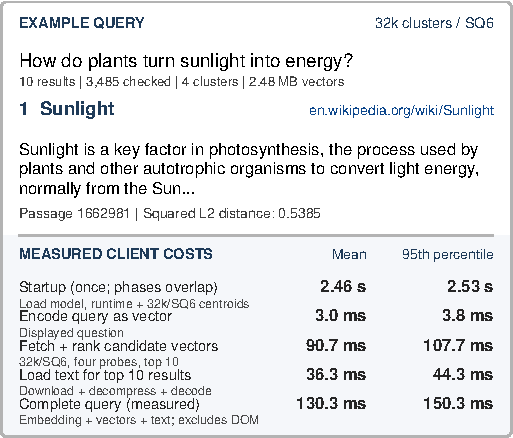
\includegraphics[width=\columnwidth]{search-example.pdf}}
\put(148.1920,153){\href{https://en.wikipedia.org/wiki/Sunlight}{\phantom{\rule{88.8080\unitlength}{10\unitlength}}}}
\end{picture}
\Description{The example question and top Wikipedia passage, with its article link, passage ID, squared L2 distance, result and cluster counts, and vector download size. The timing breakdown reports mean and 95th-percentile startup, query embedding, candidate-vector retrieval and ranking, loading text for ten results, and the directly measured complete query.}
\caption{Example query and top result, with startup, query-stage timings, and directly measured total (mean / p95; Section~\ref{sec:client-costs}).}
\label{fig:search-demo}
\end{minipage}\hfill
\begin{minipage}[t]{\columnwidth}

\centering
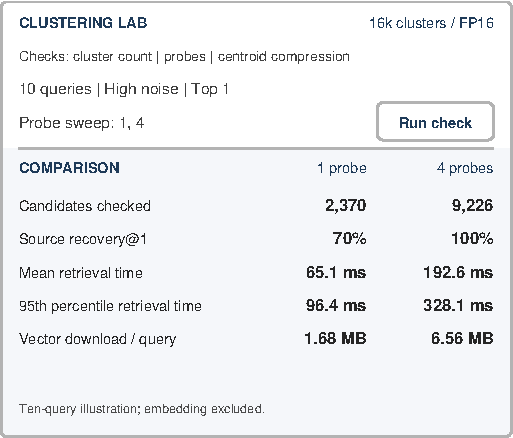
\includegraphics[width=\columnwidth]{lab-example.pdf}
\Description{Simplified clustering lab showing its three available checks, index and query settings, and a one-versus-four-probe comparison from the retained ten-query high-noise run. Rows report candidates checked, source recovery, mean and 95th-percentile retrieval times, and vector downloads per query.}
\caption{Lab walkthrough comparing one and four probes at 16k clusters, using ten high-noise queries.}
\label{fig:lab-demo}
\end{minipage}
\end{figure*}

\paragraph{Public access.}
Both pages require Internet access; search also requires WebAssembly. A poster QR code will link to the demo. The presenter will give a laptop walkthrough, with saved screenshots as a connectivity fallback. Both pages will remain public after the conference.

\Needspace{14\baselineskip}
\section{Method outline}
Figure~\ref{fig:method} traces local computation and the static files downloaded at startup and during search.

The Maloyan dataset~\cite{wiki-minilm} provides the passages and their $384$-dimensional \href{https://huggingface.co/sentence-transformers/all-MiniLM-L6-v2}{\texttt{all-MiniLM-L6-v2}} embeddings~\cite{sentence-bert,MiniLM}.

Transformers.js loads the \href{https://huggingface.co/Xenova/all-MiniLM-L6-v2}{\texttt{Xenova/all-MiniLM-L6-v2}} model in \texttt{q8} format. Queries are truncated to $256$ tokens.

\Needspace{10\baselineskip}
\subsection*{Index preparation}
We train $C$ centroids with Faiss $k$-means~\cite{Faiss}, using $20$ iterations on about $2.1$ million uniformly sampled passages. We assign each passage to its nearest centroid and store its ID and FP16 vector in that centroid's gzipped file. Centroids are published in FP16 and compressed formats; SQ6 uses six-bit scalar quantisation per component. Passage vectors remain FP16, occupying about $27$~GB before compression.

\paragraph{Result text.}
Brotli files hold $500$ passages each, except the last. The browser fetches only batches containing results and keeps decoded text in an $8$~MiB cache. Larger batches reveal less precise passage information but increase downloads.

\paragraph{Static hosting.}
The $70{,}336$ text files occupy $71$ branch deployments in the demo's Pages project, with at most $1{,}000$ data files per upload. Vectors and centroids for all three indexes occupy $59$ branches in a second project. Manifests route requests to branch URLs. Pages supports multiple active preview deployments, keeping each upload below the \href{https://developers.cloudflare.com/pages/platform/limits/}{Free-plan limit of $20{,}000$ files}. \href{https://developers.cloudflare.com/pages/functions/pricing/\#static-asset-requests}{Static-asset requests are currently free}.

\newpage
\begin{figure}[H]
\centering
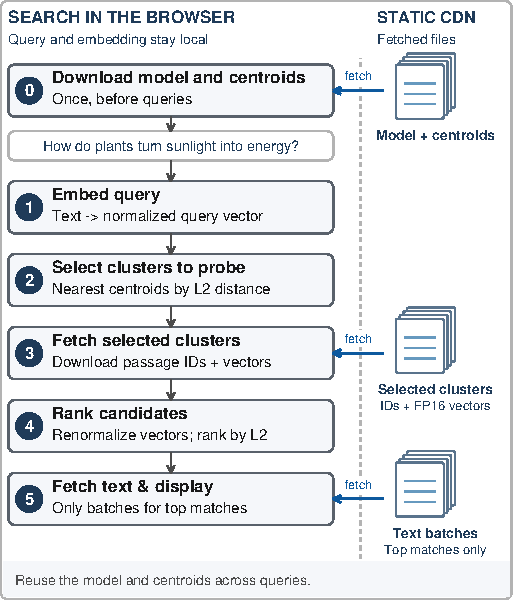
\includegraphics[width=0.98\columnwidth]{architecture.pdf}
\Description{Step zero fetches and initializes the model and centroid files once, before query processing. The question then passes through five search steps: embedding the query, selecting clusters to probe by their centroids' L2 distances, fetching the selected cluster files, renormalizing decoded passage vectors and ranking them by L2 distance to the query, and fetching text to display the top results. Arrows connect these steps. Three download arrows point from static CDN files into the browser: startup assets at initialization, passage IDs and FP16 vectors at the cluster-fetch step, and result-text batches at the final step. Loaded startup assets are reused across queries. Query text and embeddings stay local and are not uploaded.}
\caption{Local query embedding and ranking, with model and centroid downloads at startup and selective vector and text downloads per query.}
\label{fig:method}
\end{figure}

\Needspace{12\baselineskip}
\section{Supporting evaluation}
\label{sec:comparison}
All three indexes cover $35{,}167{,}920$ passage vectors. We compare routing settings using synthetic embedding perturbations and measure the complete ten-result worker workflow with a fixed question.

\paragraph{Query setup.}
All configurations share \BenchmarkQueryCount{} queries from uniformly sampled distinct source passages. We add $v\in\mathbb{R}^{384}$ with uniformly random direction and $\|v\|_2=\alpha=0.4$ to each unit-length source vector, then renormalize. We report the largest of three presets ($0.05$, $0.15$, $0.4$) to expose the probe-budget trade-off: at 32k, one-probe recovery is $97.2\%$, $93.4\%$, and $83.5\%$, respectively.

\paragraph{Perturbation scale.}
On $1{,}000$ sources, mean query-source L2 displacement is $0.378$, or $55.5\%$ of the mean nearest-neighbour distance ($0.681$) from an exact full-corpus scan excluding self matches.

\paragraph{Metric.}
\textbf{Source recovery@1} is the fraction of perturbed queries whose source passage ranks first. It measures perturbation robustness; ANN recall against exact search and question relevance are not evaluated.

\paragraph{Test environment.}
Experiments use Ubuntu~22.04 on an Intel Core i5-12400F PC with 32~GB RAM and a GTX 1660 SUPER GPU. GPU Faiss prepared the indexes. Browser experiments use Chromium~155; inference uses Transformers.js~4.3.1 with CPU-only WebAssembly and four threads. Separate \href{https://fast.com/}{FAST.com} checks reported about $300$~Mbit/s download; CDN throughput was uncontrolled.

\paragraph{Embedding compatibility.}
Re-embedding $1{,}000$ uniformly sampled passages with the q8 browser encoder yields mean and 5th-percentile cosine similarities of $0.9924$ and $0.9892$ to the stored vectors.

We compare $C\in\{8192,16384,32768\}$ with 1, 4, and 8 probes. At 32k, we sweep 1, 2, 3, 4, 6, 8, and 10 probes, and compare six centroid formats at four probes: FP16, SQ8/SQ6/SQ4~\cite{Faiss}, symmetric INT8~\cite{symmetric-int8}, and PQ4 with 4-bit codes per eight-component block~\cite{product-quantization}. Cluster assignments and FP16 passage vectors stay fixed. Shared configurations run once.

\paragraph{Hosting and timing.}
Vector and text files are fetched before timing to prime the CDN cache; the fixed-question run uses $100$ preliminary searches. Visitors need not repeat a query: earlier requests, including other visitors', can populate the CDN cache before their first search. CDN cache contents remain uncontrolled. Timed searches fetch up to ten clusters in parallel. Timed fetches bypass browser HTTP caching, and text loads also bypass the decoded-text cache; untimed accuracy checks allow cached cluster files.

\begin{samepage}
Retrieval time covers routing, cluster download, decompression, decoding, and ranking; Section~\ref{sec:client-costs} reports startup, embedding, and text loading. Each query configuration loads its centroids once. Centroid download and decoding use \BenchmarkCentroidSamples{} trials per file. Tables report mean and 95th-percentile times (p95), and vector downloads in decimal MB ($10^6$ gzipped payload bytes). Test order was not fixed.
\par
\end{samepage}

\subsection{Cluster count and probe budget}
With FP16 centroids, four probes recover over $98\%$ of source passages at all three cluster counts (Table~\ref{tab:latency-table}). More clusters reduce vector downloads and retrieval time but increase the initial centroid load.

\begin{table}[H]
\centering\normalsize\renewcommand{\arraystretch}{1.1}\setlength{\tabcolsep}{3.5pt}
\arrayrulecolor{black!25}\setlength{\arrayrulewidth}{0.3pt}
\caption{FP16 retrieval with large noise: source recovery@1, mean / p95 time, and vector downloads. Each configuration uses 10,000 queries.}
\label{tab:latency-table}
\begin{tabular}{|r|r|r|r|r|}
\hline
Clusters & Probes & Recovery (\%) & Time (ms) & MB/query\\\hline
\input figures/large-count-rows.tex
\end{tabular}
\end{table}


At 32k clusters, increasing from four to eight probes raises source recovery from $98.1\%$ to $98.8\%$, while roughly doubling retrieval time and vector downloads (Figure~\ref{fig:probes-32k}, Table~\ref{tab:latency-table}).
\begin{figure}[H]
\centering
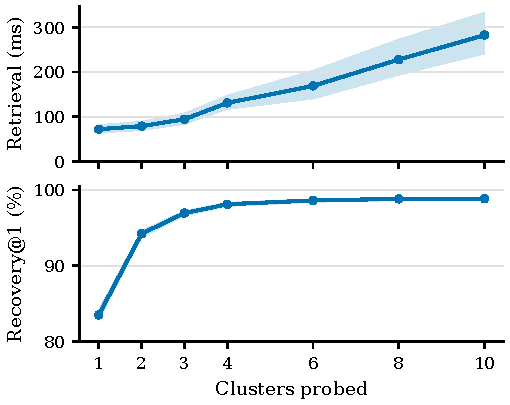
\includegraphics[width=\columnwidth]{probe-large.pdf}
\Description{Two panels plot median retrieval time in milliseconds with a 25th--75th percentile band, and source recovery@1 in percent, against probe count at 32,768 clusters with FP16 centroids and large noise.}
\caption{FP16 probe sweep at 32k clusters, large noise. Top: median retrieval time and 25th--75th percentile band. Bottom: source recovery@1. 10,000 queries per configuration.}
\label{fig:probes-32k}
\end{figure}

\subsection{Centroid loading costs}
FP16 centroid files grow from $5.81$ to $11.62$ to $23.24$~MB at 8k, 16k, and 32k clusters. Mean fetch/decode times are $106/67$, $289/129$, and $675/254$~ms, respectively, over $1{,}000$ trials per file.

Table~\ref{tab:compression-table} compares six centroid formats at 32k clusters and four probes. \textbf{SQ6 reduces mean centroid loading time from $929$~ms (FP16) to $324$~ms}, with $98.1\%$ recovery for both.

\begin{table}[tb]
\centering\normalsize\renewcommand{\arraystretch}{1.2}\setlength{\tabcolsep}{3.5pt}
\arrayrulecolor{black!25}\setlength{\arrayrulewidth}{0.3pt}
\caption{Centroid formats at 32k clusters and four probes: source recovery@1 on $10{,}000$ queries ($\alpha=0.4$), file size, and loading mean / p95 over 1,000 trials per file. Decode includes gzip decompression.}
\label{tab:compression-table}
\begin{tabular}{|l|c|c|c|c|}
\hline
Format & Recovery (\%) & Size (MB) & Fetch (ms) & Decode (ms)\\\hline
\input figures/large-compression-rows.tex
\end{tabular}
\end{table}


SQ8 and INT8 give similar recovery with larger files; SQ4 and PQ4 trade recovery for smaller files.

These results motivate 32k/SQ6 and four probes: reduced vector downloads and centroid loading costs with high recovery.

\subsection{Client setup and query costs}
\label{sec:client-costs}
\paragraph{Complete ten-result query.}
For ``How do plants turn sunlight into energy?'', the client returns ten passages at 32k/SQ6 and four probes. Across $1{,}000$ repetitions, search submission to worker reply takes $130.3/150.3$~ms (mean/p95), including embedding, vector retrieval, text loading, and message handling. Startup and DOM rendering are excluded; model and decoded centroids stay loaded. The results require $2.48$~MB of gzipped vectors and $0.77$~MB of Brotli text ($3.25$~MB total payload, excluding HTTP headers).

\paragraph{Separate components.}
For synthetic queries, top-1 retrieval at 32k/SQ6 and four probes takes $122/187$~ms (mean/p95), with $98.1\%$ source recovery.
\paragraph{Query embedding.}
Embedding takes $9.1/9.5$~ms (mean/p95) at $64$ tokens, $16.9/17.3$~ms at $128$, and $33.8/34.5$~ms at $256$. We time $1{,}000$ calls over $100$ passages, following three untimed calls per length.

\paragraph{Result text.}
Loading text for ten results averages $34.9$~ms (p95 $54.9$~ms), including download, decompression, and decoding. We time $1{,}000$ groups drawn from $10{,}000$ distinct sampled passages.

\paragraph{Startup.}
Startup spans worker creation until the model and 32k SQ6 centroids are ready, excluding page navigation. Across $100$ fresh browser contexts, it takes $2.46/2.53$~s (mean/p95). The model ($23.7$~MB), WebAssembly runtime ($14.3$~MB), and centroids ($9.0$~MB) total about $47$~MB. Browser caching is bypassed; loading phases overlap.

\subsection{Discussion}
Selective downloads trade per-query bandwidth for avoiding a full local index: the synthetic workload averages $3.98$~MB of vectors per query, excluding text. The interactive client reuses its model and centroids, allows browser HTTP caching of vectors, and retains decoded text in its bounded cache. Model files can persist in browser storage. Repeated queries can therefore transfer less data than the cache-bypassed benchmarks.

\section{Conclusion}
Local IVF routing enables browser search over $35.2$ million passages through selective downloads from static hosting. The search page and lab expose how clustering, probing, and centroid compression affect source recovery, latency, and bandwidth.

\section{Ethical use of data}
The demo reuses public Wikipedia passages and embeddings from the cited dataset~\cite{wiki-minilm}. Passages reflect an archived snapshot and may be outdated or biased; linked articles may have changed or been deleted. Experiments use sampled passages and synthetic embedding perturbations, with no human-participant study. Queries and embeddings stay local, but file-request patterns may reveal search interests.

\bibliography{ref}
\bibliographystyle{ACM-Reference-Format}

\end{document}
